\documentclass[conference]{IEEEtran}
\usepackage[left=1.57cm,right=1.57cm,top=2.5cm,bottom=3cm,headsep=1cm,footskip=1.5cm]{geometry}
\IEEEoverridecommandlockouts
% The preceding line is only needed to identify funding in the first footnote. If that is unneeded, please comment it out.
%\usepackage[english]{babel}
\usepackage{amsmath,amssymb,amsfonts}
\usepackage{graphicx}
\usepackage{subcaption}
\usepackage[dvipsnames]{xcolor}
\usepackage{fancyhdr}
\usepackage{lipsum}
\usepackage{tabularx}
\usepackage{titlesec}
\usepackage[labelsep=period]{caption}
\usepackage{multirow}
\usepackage{indentfirst}
\usepackage{xpatch}
\usepackage{setspace}
\usepackage{times} 
%\usepackage{slashbox}
\usepackage{enumitem}
\usepackage{gensymb}
\usepackage{cite}
\usepackage{color,soul}
\usepackage[font=small]{caption}
\usepackage[labelfont={color=RoyalBlue}]{caption}
\captionsetup[table]{skip=6pt}
\renewcommand\IEEEkeywordsname{\textcolor{RoyalBlue}{Keywords}}
\renewcommand\abstractname{\textcolor{RoyalBlue}{Abstract}}

\def\BibTeX{{\rm B\kern-.05em{\sc i\kern-.025em b}\kern-.08em
    T\kern-.1667em\lower.7ex\hbox{E}\kern-.125emX}}

%%%%%%%%%%% CITE IJRCS %%%%%%%%%%%
\renewcommand{\citeleft}{\textcolor{RoyalBlue}{[}}
\renewcommand{\citeright}{\textcolor{RoyalBlue}{]}}

\def\citepunct{\textcolor{RoyalBlue}{]}, \textcolor{RoyalBlue}{[}}
\def\citedash{\textcolor{RoyalBlue}{]}--\textcolor{RoyalBlue}{[}}
%%%%%%%%%%% CITE IJRCS %%%%%%%%%%%

\usepackage{url}
\usepackage{hyperref}
\hypersetup{
	colorlinks=true,
	linkcolor=RoyalBlue,      
	urlcolor=RoyalBlue,
	citecolor=RoyalBlue,
	citebordercolor=0 0 1
}
\urlstyle{same}

%\addto\captionsenglish{\renewcommand{\figurename}{\textbf{Fig.}}}
%\addto\captionsenglish{\renewcommand{\tablename}{\textbf{Table}}}

\renewcommand{\tablename}{\textcolor{RoyalBlue}{TABLE}}
\renewcommand{\figurename}{\textcolor{RoyalBlue}{Fig.}}

\usepackage{tabularx}
\newcolumntype{R}{>{\raggedright\arraybackslash}X}
%Unt uk membuat p e r i n t a h r a t a k i r i
\newcolumntype{L}{>{\raggedleft\arraybackslash}X}
%Unt uk membuat p e r i n t a h r a t a k ana n
\newcolumntype{C}{>{\centering\arraybackslash}X}
%Unt uk membuat p e r i n t a h r a t a t e ng ah

\usepackage{float}

\usepackage[labelsep=period, justification=centering, font=scriptsize]{caption}
\usepackage{enumitem}
\setlist{nolistsep}
\captionsetup{singlelinecheck=off} %bair caption rata kiri

\setlength{\parskip}{0.3em} %spasi after before

\renewcommand{\headrulewidth}{1.5pt}
\xpretocmd\headrule{\color{RoyalBlue}}{}{\PatchFailed}

\renewcommand{\footrulewidth}{1.5pt}
\renewcommand{\footrule}{\hbox to\headwidth{%
		\color{RoyalBlue}\leaders\hrule height \headrulewidth\hfill}}

\titlespacing{\section}{0pt}{12pt}{4pt}
\titleformat{\section}[hang]{\centering\scshape}{\textcolor{RoyalBlue}{\thesection. }}{0.5em}{\color{RoyalBlue}}

\titlespacing{\subsection}{0pt}{6pt}{3pt}
\titleformat{\subsection}[hang]{\normalfont\itshape}{\textcolor{RoyalBlue}{\thesubsectiondis }}{0.5em}{\color{RoyalBlue}}
%\titlespacing{\subsection}{0pt}{6pt}{3pt}
%\titleformat{\subsection}[hang]{\centering\scshape}{\textcolor{RoyalBlue}{\thesubsection. }}{0.5em}{\color{RoyalBlue}}
%\titlespacing{\subsection}{0pt}{6pt}{3pt}
%\titleformat{\subsection}[hang]{\bfseries}{\thesubsection. }{0.75em}{}
%\titlespacing{\subsection}{0pt}{6pt}{3pt}
%\titleformat{\subsection}[hang]{\normalfont\itshape}{\textcolor{RoyalBlue}{\thesubsectiondis. }}{0.5em}{\color{RoyalBlue}}

\usepackage{fancyhdr}
\usepackage{comment}

\fancypagestyle{firstpage}{
\fancyhf{}
\fancyhead[L]{Control Systems and Optimization Letters, Vol. 2, No 1, 2024\\
ISSN: 2985-6116, DOI: 10.59247/csol.vxix.xx}
\fancyhead[R]{\thepage}          
%\fancyfoot[L]{\includegraphics{open_access}}
\fancyfoot[C]{\footnotesize This work is licensed under a Creative Commons Attribution 4.0 License. For more information, see \url{https://creativecommons.org/licenses/by/4.0/}
}
%\fancyfoot[R]{Journal Email: jrc@umy.ac.id}
\renewcommand{\footrulewidth}{0.7pt} 
\renewcommand{\headrulewidth}{0.7pt}
}

\fancypagestyle{followingpage}{
\fancyhf{}
\fancyhead[L]{Control Systems and Optimization Letters, Vol. 2, No 1, 2024}
%\fancyhead[C]{ISSN: 2715-5072}
\fancyhead[R]{\thepage}
\fancyfoot[C]{\small  First Author Name (Title)}
\renewcommand{\headrulewidth}{0.7pt}
\renewcommand{\footrulewidth}{0.7pt}
}

\AtBeginDocument{\thispagestyle{firstpage}}
\pagestyle{followingpage}

\setcounter{page}{1}

\usepackage{tikz}
\usetikzlibrary{arrows.meta,positioning}

% ---------------------------------------------------------------
% DRAFT (acuan). Yellow-highlighted [..] = to be filled after the
% experiments or methodological decisions. Do not cite numbers that
% are still highlighted.
% ---------------------------------------------------------------
\newcommand{\tbd}[1]{\hl{[#1]}}

\begin{document}

\title{\textcolor{RoyalBlue}{Comparative Evaluation of YOLOv8-OBB and YOLO11-OBB for Oriented Ship Detection in Sentinel-1 SAR Imagery of the Makassar Strait}
}

\author{\small Author \textsuperscript{1} , Author \textsuperscript{2} , Author \textsuperscript{3} , Author \textsuperscript{4} , Author \textsuperscript{5,*}
	\\
	\textsuperscript{1, 2, 3, 4, 5} Department of Electrical Engineering, Universitas Ahmad Dahlan, Yogyakarta, Indonesia\\
	Email: \textsuperscript{1} author@email, \textsuperscript{2} author@email, \textsuperscript{3} author@email, \textsuperscript{4} author@email, \textsuperscript{5} author@email\\
	Orcid: \textsuperscript{1} Orcid URL, \textsuperscript{2} Orcid URL, \textsuperscript{3} Orcid URL, \textsuperscript{4} Orcid URL, \textsuperscript{5} Orcid URL\\
	*Corresponding Author}

\maketitle

\begin{abstract}
Monitoring vessel activity along the Indonesian Archipelagic Sea Lane II, of which the Makassar Strait is a principal corridor, requires observations that do not depend on daylight, cloud-free conditions, or cooperative reporting by ships. Spaceborne synthetic aperture radar provides such observations, but automatic ship detection in radar images is hampered by speckle, sea clutter, small target size, and arbitrary ship orientation. This study presents a controlled comparison of two oriented bounding box detectors, YOLOv8-OBB and YOLO11-OBB, for ship detection in Sentinel-1 imagery, and examines how both models behave when applied to scenes of the Makassar Strait. Both models were trained and evaluated on the Dual-Polarimetric SAR Ship Detection Dataset, which contains 1,236 image chips with 3,540 ship instances annotated with rotated boxes, using identical data splits, input sizes, training schedules, augmentation settings, and hardware. Detection quality was measured with precision, recall, F1-score, mAP at an intersection over union threshold of 0.5, and mAP averaged over thresholds from 0.5 to 0.95, while efficiency was measured with parameter count, computational cost, and inference speed. \hl{[RESULTS: YOLOv8-OBB achieved an mAP50 of XX and YOLO11-OBB an mAP50 of XX; summarise the main difference in accuracy and speed in one or two sentences.]} \hl{[APPLICATION: summarise what the detections on the Makassar Strait scenes show, including typical false alarms and missed ships.]} The results provide empirical evidence on the strengths and limitations of both detectors and on the effect of transferring a model trained on a public dataset to an operational study area, supporting the development of automated maritime monitoring in Indonesian waters.
\end{abstract}

\begin{IEEEkeywords}
\textit{Ship detection; Synthetic aperture radar; Sentinel-1; Oriented bounding box; YOLOv8; YOLO11; Makassar Strait}
\end{IEEEkeywords}

%=================================================================
\section{INTRODUCTION}
% P1 -- maritime monitoring in Indonesia
As the world's largest archipelagic state, Indonesia relies on its sea lanes for domestic connectivity, international trade, and the exercise of maritime sovereignty. Continuous and reliable monitoring of vessel activity is therefore a basic requirement for maritime surveillance, navigational safety, fisheries management, and law enforcement \cite{wuryantari2026,putra2026}. Cooperative reporting systems such as the Automatic Identification System (AIS) are widely used to analyse vessel behaviour \cite{shanthi2022}, but they only capture vessels that carry and operate a transponder. Vessels that do not transmit, often referred to as dark vessels, can only be observed by independent sensors, which has motivated the use of satellite imagery and its fusion with AIS for maritime surveillance \cite{rodger2020,liu2022ais,kerekes2024,kim2025dark,albaqami2026}.

% P2 -- Makassar Strait and ALKI II
The Makassar Strait is one of the principal corridors of the Indonesian Archipelagic Sea Lane II (ALKI II), which connects the Sulawesi Sea in the north with the Flores Sea and the Lombok Strait in the south \cite{yulia2023}. The strait is regarded as a strategic route for international navigation \cite{rlj2022}, it is subject to interregional marine spatial planning \cite{yulia2023}, and the security of the ALKI corridors is a recurring concern of national defence and border management \cite{silalahi2026,wuryantari2026}. These characteristics make the Makassar Strait a relevant study area for automated ship monitoring.

% P3 -- Sentinel-1 SAR
Synthetic aperture radar (SAR) is well suited to this task because, as an active microwave sensor, it acquires images independently of solar illumination and largely independently of cloud cover and weather conditions. The Sentinel-1 mission of the Copernicus programme provides C-band SAR data with systematic global coverage and open access \cite{torres2012}, and its suitability for ship detection has been assessed against other spaceborne SAR systems \cite{velotto2015}. Nevertheless, SAR images differ fundamentally from optical images: their appearance depends on radar backscattering, imaging geometry, and polarization rather than on visible colour and texture, which limits the direct transfer of methods developed for optical imagery.

% P4 -- technical challenges and traditional methods
Ship detection in SAR images faces several well-documented difficulties \cite{li2022review}. Speckle noise degrades image quality and complicates the interpretation of fine structures \cite{zhang2023speckle}, while sea clutter, whose intensity varies with sea state and wind, can produce bright responses that resemble ships. Many ships occupy only a few pixels in medium-resolution products such as Sentinel-1, which makes small-target detection particularly challenging \cite{zhang2020lsssdd}. Ships near ports and coastlines are surrounded by strong scatterers from land structures, which increases false alarms in inshore scenes \cite{yao2026fsmd,wang2026fsp}. Traditional detectors based on the constant false alarm rate (CFAR) principle model the statistics of the sea background and remain widely studied \cite{li2022cfar,zhang2021cfar}, but their performance depends on the validity of the clutter model and degrades in heterogeneous backgrounds or under interference \cite{ma2022cfar}.

% P5 -- deep learning detectors and datasets
Deep learning has progressively replaced handcrafted pipelines in SAR ship detection \cite{li2022review}. Two-stage detectors such as Faster R-CNN generate region proposals before classification \cite{ren2017}, whereas one-stage detectors predict boxes and classes in a single pass and offer a more favourable trade-off between accuracy and speed \cite{redmon2016}. Multi-scale feature fusion through feature pyramids \cite{lin2017fpn} and path aggregation \cite{liu2018panet} has become a standard component of modern detectors. Progress has been supported by public SAR datasets, including SSDD \cite{zhang2021ssdd}, the SAR-Ship-Dataset \cite{wang2019sard}, HRSID \cite{wei2020hrsid}, and LS-SSDD-v1.0 \cite{zhang2020lsssdd}. Building on these datasets, researchers have proposed anchor-free detectors \cite{jiang2021rcenter,yao2022atsd,peng2022yolox}, lightweight networks \cite{yan2022lssdet}, multi-scale attention and dynamic feature fusion \cite{wan2026msadet,cao2025dmff}, and transformer-based architectures for small or complex targets \cite{yu2025smep,li2025fant}.

% P6 -- YOLO family in SAR ship detection
The You Only Look Once (YOLO) family has become a popular baseline for SAR ship detection because of its efficiency. Earlier work adapted YOLOv5 with lightweight modules or bidirectional feature pyramids \cite{pang2022mne,yu2024bifpn}, and other studies designed lightweight YOLO variants for multi-scale targets \cite{guo2022lmsd,ren2023yololite}. More recently, YOLOv8 \cite{yolov8} has been modified for efficient, lightweight, and small-target SAR ship detection \cite{he2024yolov8sar,niu2024ltyolov8,gao2025styolov8,wei2024flyolov8}, and YOLO11 \cite{yolo11} has been extended with attention, multi-scale, and lightweight designs \cite{li2026acmix,li2025esd,yin2026sla}. Comparative analyses of YOLO models on several SAR datasets have also been reported \cite{cavli2025}. Most of these studies, however, use horizontal bounding boxes and evaluate modified architectures on high-resolution benchmarks.

% P7 -- oriented bounding boxes
Horizontal bounding boxes describe elongated, arbitrarily oriented ships poorly: they enclose substantial background and overlap strongly when ships are moored side by side. Oriented bounding box (OBB) detection, popularised for aerial images by the DOTA benchmark \cite{xia2018dota} and reviewed extensively for rotated objects \cite{he2024rotsurvey}, describes each object by its centre, dimensions, and rotation angle. In SAR ship detection, rotated annotations are provided by datasets such as SRSDD-v1.0 \cite{lei2021srsdd}, and several studies have addressed the representation and encoding of rotated boxes \cite{zhao2021afobb,guo2023border,jiang2023ledrbe,li2025obbcont} as well as lightweight and feature-enhanced oriented detectors \cite{meng2024lsrdet,zhang2025pde,huang2024lwyolo11}. Both YOLOv8 and YOLO11 provide native OBB variants \cite{yolov8,yolo11}, which makes them practical candidates for operational oriented ship detection.

% P8 -- DSSDD and dual polarization
Polarimetric information offers an additional cue for distinguishing ships from clutter. The Dual-Polarimetric SAR Ship Detection Dataset (DSSDD) was built from 50 Sentinel-1 interferometric wide-swath single-look complex (SLC) images in VV and VH polarizations; it contains 1,236 image chips of $256 \times 256$ pixels with 3,540 ship instances annotated with both rotated and horizontal bounding boxes \cite{hu2021dssdd}. Dual-polarization feature fusion and enhancement networks have shown that combining both channels can benefit ship detection \cite{xu2023gwfr,li2023dpfe}. Because DSSDD is derived from Sentinel-1 and provides rotated annotations, it is a natural basis for training OBB detectors intended for Sentinel-1 data over Indonesian waters.

% P9 -- research gap
Two practical questions remain open for applying OBB detectors to maritime monitoring in Indonesian waters. First, a controlled comparison between YOLOv8-OBB and YOLO11-OBB on a dual-polarization Sentinel-1 dataset, using identical data splits, input sizes, training schedules, and hardware, is needed to determine whether the newer architecture offers a meaningful benefit for SAR ship detection rather than relying on results from optical benchmarks. Second, a model trained on a public dataset must be examined on scenes from the target area, because differences in acquisition conditions, product type, and sea state can cause a domain shift, a problem that has motivated a growing body of domain adaptation research for SAR ship detection \cite{liu2023da,tu2025mamba,zhang2025sfda,wang2026o2s}.
% TODO: validate this gap against a full literature search before submission.

% P10 -- contributions
This study addresses these questions through a comparative experimental evaluation of YOLOv8-OBB and YOLO11-OBB for ship detection in Sentinel-1 SAR images. The contributions of this paper are as follows: (1) both models are trained and evaluated on DSSDD under a consistent experimental protocol; (2) their performance is compared in terms of precision, recall, F1-score, mAP@50, mAP@50:95, model complexity, and inference speed; and (3) both models are applied to Sentinel-1 scenes of the Makassar Strait within ALKI II, and the resulting detections are analysed to identify the strengths and limitations of each model for maritime monitoring in the study area. The remainder of this paper is organised as follows. Section II describes the data, models, and experimental protocol; Section III presents and discusses the results; and Section IV concludes the paper.

%=================================================================
\section{METHODS}
\subsection{Research Workflow}
The research workflow is shown in \textcolor{RoyalBlue}{Fig.} \ref{fig:workflow}. It consists of two branches. In the benchmark branch, DSSDD is converted into the YOLO-OBB annotation format, split into training, validation, and test subsets, and used to train and evaluate both models under the same protocol. In the application branch, Sentinel-1 scenes of the Makassar Strait are preprocessed into the same input representation, tiled, and passed to both trained models, after which the detections are merged and analysed.

\begin{figure}[h]
	\centering
	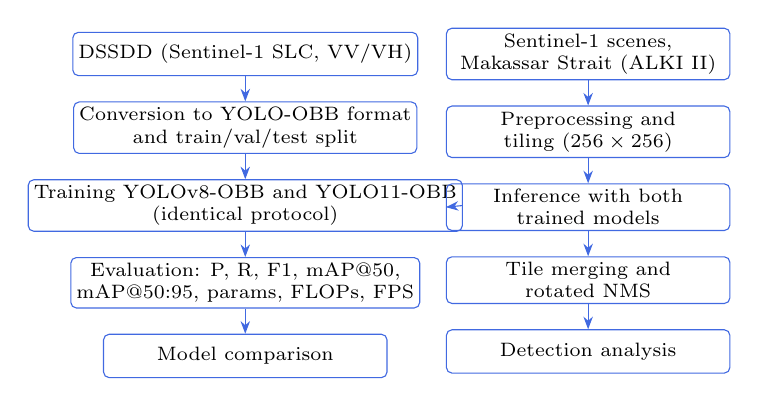
\begin{tikzpicture}[
		node distance=0.32cm and 0.35cm,
		box/.style={draw=RoyalBlue, rounded corners=2pt, align=center, font=\scriptsize, minimum width=3.6cm, minimum height=0.55cm, inner sep=2pt},
		arr/.style={-{Stealth[length=1.6mm]}, RoyalBlue}]
		\node[box] (d) {DSSDD (Sentinel-1 SLC, VV/VH)};
		\node[box, below=of d] (p) {Conversion to YOLO-OBB format\\ and train/val/test split};
		\node[box, below=of p] (t) {Training YOLOv8-OBB and YOLO11-OBB\\ (identical protocol)};
		\node[box, below=of t] (e) {Evaluation: P, R, F1, mAP@50,\\ mAP@50:95, params, FLOPs, FPS};
		\node[box, below=of e] (c) {Model comparison};
		\node[box, right=of d] (s) {Sentinel-1 scenes,\\ Makassar Strait (ALKI II)};
		\node[box, below=of s] (sp) {Preprocessing and\\ tiling ($256 \times 256$)};
		\node[box, below=of sp] (i) {Inference with both\\ trained models};
		\node[box, below=of i] (m) {Tile merging and\\ rotated NMS};
		\node[box, below=of m] (a) {Detection analysis};
		\draw[arr] (d) -- (p); \draw[arr] (p) -- (t); \draw[arr] (t) -- (e); \draw[arr] (e) -- (c);
		\draw[arr] (s) -- (sp); \draw[arr] (sp) -- (i); \draw[arr] (i) -- (m); \draw[arr] (m) -- (a);
		\draw[arr] (t.east) -- (i.west);
	\end{tikzpicture}
	\caption{Research workflow of this study.}
	\label{fig:workflow}
\end{figure}

\subsection{Dataset}
DSSDD \cite{hu2021dssdd} was constructed from 50 Sentinel-1 interferometric wide-swath SLC images acquired in VV and VH polarizations. The images were cropped into 1,236 chips of $256 \times 256$ pixels containing 3,540 ship instances. Each ship is annotated with both a rotated bounding box and a horizontal bounding box, and the chips are provided as pseudo-colour images that encode the polarimetric information. Only the rotated annotations are used in this study. The main properties of the dataset are summarised in \textcolor{RoyalBlue}{Table} \ref{tab:dataset}. The chips are divided into training, validation, and test subsets with a ratio of \tbd{e.g. 70:10:20, or the original DSSDD split if provided}; the same split is used for both models.

\begin{table}[h!]
	\centering
	\caption{SUMMARY OF THE DSSDD DATASET}
	\begin{footnotesize}
	\begin{tabular}{ll}
		\hline
		\textbf{Property} & \textbf{Value} \\
		\hline
		Sensor and mode & Sentinel-1, IW \\
		Product & Single-look complex (SLC) \\
		Polarization & VV and VH \\
		Source images & 50 \\
		Image chips & 1,236 \\
		Chip size & $256 \times 256$ pixels \\
		Ship instances & 3,540 \\
		Annotation & Rotated and horizontal boxes \\
		Training / validation / test chips & \tbd{-- / -- / --} \\
		\hline
	\end{tabular}
	\label{tab:dataset}
	\end{footnotesize}
\end{table}

\subsection{Study Area and Sentinel-1 Data}
The study area is the Makassar Strait between Kalimantan and Sulawesi, which forms the northern part of ALKI II \cite{yulia2023}. \tbd{Specify the bounding coordinates of the area of interest.} Sentinel-1 scenes covering the strait were obtained from the Copernicus data space. The acquisitions used in this study are listed in \textcolor{RoyalBlue}{Table} \ref{tab:scenes}. \tbd{Decide whether SLC or GRD products are used. If GRD is used, state that the complex phase information available in DSSDD is not available and describe how the pseudo-colour representation is reproduced from the VV and VH intensities.}

\begin{table}[h!]
	\centering
	\caption{SENTINEL-1 SCENES OF THE MAKASSAR STRAIT}
	\begin{footnotesize}
	\begin{tabular}{cccc}
		\hline
		\textbf{No.} & \textbf{Acquisition date} & \textbf{Product} & \textbf{Polarization} \\
		\hline
		1 & \tbd{dd-mm-yyyy} & \tbd{SLC/GRD} & VV+VH \\
		2 & \tbd{dd-mm-yyyy} & \tbd{SLC/GRD} & VV+VH \\
		\hline
	\end{tabular}
	\label{tab:scenes}
	\end{footnotesize}
\end{table}

\subsection{Preprocessing}
The rotated annotations of DSSDD are converted into the YOLO-OBB format, in which each object is written as a class index followed by the four corner coordinates of its rotated box, normalised by the image width and height. For a box with centre $(x_c, y_c)$, width $w$, height $h$, and angle $\theta$, the corners are obtained by
\begin{equation}
	\begin{bmatrix} x_i \\ y_i \end{bmatrix} =
	\begin{bmatrix} x_c \\ y_c \end{bmatrix} +
	\begin{bmatrix} \cos\theta & -\sin\theta \\ \sin\theta & \cos\theta \end{bmatrix}
	\begin{bmatrix} \delta_{x,i}\, w/2 \\ \delta_{y,i}\, h/2 \end{bmatrix},
	\label{eq:corners}
\end{equation}
where $(\delta_{x,i}, \delta_{y,i}) \in \{(-1,-1), (1,-1), (1,1), (-1,1)\}$ for $i = 1, \dots, 4$.

The Sentinel-1 scenes of the study area are processed with \tbd{SNAP or other software}: \tbd{list the steps, e.g. orbit correction, radiometric calibration, land masking, and conversion to the DSSDD pseudo-colour representation}. Each processed scene is divided into $256 \times 256$ tiles with an overlap of \tbd{XX} pixels so that ships on tile borders are not lost.

\subsection{Detection Models}
YOLOv8 \cite{yolov8} uses a CSP-based backbone built from C2f modules and a spatial pyramid pooling fast (SPPF) block, a neck that combines feature pyramid and path aggregation structures \cite{lin2017fpn,liu2018panet}, and an anchor-free decoupled head. YOLO11 \cite{yolo11} retains this overall structure but replaces the C2f modules with C3k2 blocks and adds a C2PSA block with position-sensitive spatial attention after the SPPF layer. In the OBB variants of both models, the detection head predicts an additional rotation angle for each box, so that the output is a rotated rectangle instead of a horizontal one. The main differences are summarised in \textcolor{RoyalBlue}{Table} \ref{tab:models}. Both models are initialised from the OBB weights released by Ultralytics, which were pretrained on the DOTA dataset \cite{xia2018dota}. \tbd{State the model scale used, e.g. nano (n) or small (s), and use the same scale for both models.}

\begin{table}[h!]
	\centering
	\caption{COMPARISON OF THE EVALUATED MODELS}
	\begin{footnotesize}
	\begin{tabular}{lcc}
		\hline
		\textbf{Component} & \textbf{YOLOv8-OBB} & \textbf{YOLO11-OBB} \\
		\hline
		Backbone block & C2f & C3k2 \\
		Attention block & -- & C2PSA \\
		Neck & FPN + PAN & FPN + PAN \\
		Head & Anchor-free, decoupled & Anchor-free, decoupled \\
		Box output & $(x_c, y_c, w, h, \theta)$ & $(x_c, y_c, w, h, \theta)$ \\
		Parameters (M) & \tbd{--} & \tbd{--} \\
		FLOPs (G) & \tbd{--} & \tbd{--} \\
		\hline
	\end{tabular}
	\label{tab:models}
	\end{footnotesize}
\end{table}

Both models are trained with the same composite loss,
\begin{equation}
	\mathcal{L} = \lambda_{box}\mathcal{L}_{box} + \lambda_{cls}\mathcal{L}_{cls} + \lambda_{dfl}\mathcal{L}_{dfl},
	\label{eq:loss}
\end{equation}
where $\mathcal{L}_{box}$ is the rotated box regression loss, $\mathcal{L}_{cls}$ is the binary cross-entropy classification loss, $\mathcal{L}_{dfl}$ is the distribution focal loss, and the weights are kept at the default values $\lambda_{box} = 7.5$, $\lambda_{cls} = 0.5$, and $\lambda_{dfl} = 1.5$ for both models.

\subsection{Experimental Setup}
To ensure a fair comparison, both models are trained with identical settings, listed in \textcolor{RoyalBlue}{Table} \ref{tab:train}. The same random seed, data split, augmentation pipeline, and hardware are used, and the checkpoint with the best validation mAP@50:95 is used for testing.

\begin{table}[h!]
	\centering
	\caption{TRAINING CONFIGURATION (IDENTICAL FOR BOTH MODELS)}
	\begin{footnotesize}
	\begin{tabular}{ll}
		\hline
		\textbf{Setting} & \textbf{Value} \\
		\hline
		Framework & Ultralytics \tbd{version} \\
		Input size & \tbd{256 or 640} pixels \\
		Epochs & \tbd{e.g. 300} \\
		Batch size & \tbd{e.g. 16} \\
		Optimizer & \tbd{SGD / AdamW} \\
		Initial learning rate & \tbd{e.g. 0.01} \\
		Augmentation & \tbd{default Ultralytics pipeline} \\
		Random seed & \tbd{e.g. 0} \\
		Hardware & \tbd{GPU, CPU, RAM} \\
		\hline
	\end{tabular}
	\label{tab:train}
	\end{footnotesize}
\end{table}

\subsection{Evaluation Metrics}
A prediction is counted as a true positive ($TP$) if its rotated intersection over union with a ground-truth box,
\begin{equation}
	\mathrm{IoU}_r = \frac{\left| B_p \cap B_g \right|}{\left| B_p \cup B_g \right|},
	\label{eq:iou}
\end{equation}
exceeds the threshold, where $B_p$ and $B_g$ are the predicted and ground-truth rotated boxes. Unmatched predictions are false positives ($FP$) and unmatched ground-truth boxes are false negatives ($FN$). Precision, recall, and F1-score are defined as
\begin{equation}
	P = \frac{TP}{TP + FP}, \quad R = \frac{TP}{TP + FN}, \quad F1 = \frac{2PR}{P + R}.
	\label{eq:prf}
\end{equation}
The average precision is the area under the precision--recall curve,
\begin{equation}
	AP = \int_{0}^{1} P(R)\, dR.
	\label{eq:ap}
\end{equation}
Because the task has a single class, mAP equals AP. We report mAP@50, computed at $\mathrm{IoU}_r = 0.5$, and mAP@50:95, the mean AP over thresholds from 0.50 to 0.95 in steps of 0.05. Efficiency is reported as the number of parameters, floating-point operations, and inference speed,
\begin{equation}
	FPS = \frac{1000}{t_{pre} + t_{inf} + t_{post}},
	\label{eq:fps}
\end{equation}
where $t_{pre}$, $t_{inf}$, and $t_{post}$ are the preprocessing, inference, and postprocessing times per image in milliseconds.

\subsection{Application to the Makassar Strait}
Both trained models are applied to the tiled Sentinel-1 scenes with a confidence threshold of \tbd{e.g. 0.25}. Detections from overlapping tiles are mapped back to scene coordinates and merged with rotated non-maximum suppression. \tbd{If reference labels are available for the study area, evaluate the detections with the metrics above. Otherwise, restrict the analysis to visual inspection, detection counts, and optionally a comparison with AIS records, and do not report accuracy for the study area.}

%=================================================================
\section{RESULTS AND DISCUSSION}
\subsection{Training Behaviour}
\textcolor{RoyalBlue}{Fig.} \ref{fig:curves} shows the training and validation curves of both models. \tbd{Describe convergence speed, the epoch of the best checkpoint, and any sign of overfitting.}

\begin{figure}[h]
	\centering
	\fbox{\parbox[c][3.2cm][c]{0.9\columnwidth}{\centering\footnotesize [Placeholder: loss and validation mAP@50:95 curves of YOLOv8-OBB and YOLO11-OBB]}}
	\caption{Training loss and validation mAP@50:95 of both models.}
	\label{fig:curves}
\end{figure}

\subsection{Detection Performance on DSSDD}
\textcolor{RoyalBlue}{Table} \ref{tab:results} compares the detection performance of both models on the DSSDD test set. \tbd{Report which model achieves higher mAP@50 and mAP@50:95, and by how much. Discuss whether the difference comes mainly from precision (fewer false alarms) or recall (fewer missed ships). If several runs with different seeds are performed, report mean and standard deviation.}

\begin{table}[h!]
	\centering
	\caption{DETECTION PERFORMANCE ON THE DSSDD TEST SET}
	\begin{footnotesize}
	\begin{tabular}{lccccc}
		\hline
		\textbf{Model} & \textbf{P} & \textbf{R} & \textbf{F1} & \textbf{mAP@50} & \textbf{mAP@50:95} \\
		\hline
		YOLOv8-OBB & \tbd{--} & \tbd{--} & \tbd{--} & \tbd{--} & \tbd{--} \\
		YOLO11-OBB & \tbd{--} & \tbd{--} & \tbd{--} & \tbd{--} & \tbd{--} \\
		\hline
	\end{tabular}
	\label{tab:results}
	\end{footnotesize}
\end{table}

\subsection{Computational Efficiency}
\textcolor{RoyalBlue}{Table} \ref{tab:eff} lists the model complexity and inference speed measured on \tbd{hardware}. \tbd{Discuss the accuracy--speed trade-off and its relevance for processing full Sentinel-1 scenes.}

\begin{table}[h!]
	\centering
	\caption{MODEL COMPLEXITY AND INFERENCE SPEED}
	\begin{footnotesize}
	\begin{tabular}{lccc}
		\hline
		\textbf{Model} & \textbf{Params (M)} & \textbf{FLOPs (G)} & \textbf{FPS} \\
		\hline
		YOLOv8-OBB & \tbd{--} & \tbd{--} & \tbd{--} \\
		YOLO11-OBB & \tbd{--} & \tbd{--} & \tbd{--} \\
		\hline
	\end{tabular}
	\label{tab:eff}
	\end{footnotesize}
\end{table}

\subsection{Qualitative Analysis}
\textcolor{RoyalBlue}{Fig.} \ref{fig:qual} shows representative detections on test chips containing offshore ships, densely clustered ships, and inshore ships. \tbd{Describe typical errors: false alarms from clutter or land structures, missed small ships, merged boxes for adjacent ships, and inaccurate angles.} These observations can be related to the challenges of small targets \cite{zhang2020lsssdd} and complex inshore backgrounds \cite{yao2026fsmd} reported in previous studies.

\begin{figure}[h]
	\centering
	\fbox{\parbox[c][3.2cm][c]{0.9\columnwidth}{\centering\footnotesize [Placeholder: ground truth, YOLOv8-OBB, and YOLO11-OBB detections on representative DSSDD test chips]}}
	\caption{Examples of detection results on the DSSDD test set.}
	\label{fig:qual}
\end{figure}

\subsection{Application to the Makassar Strait}
\textcolor{RoyalBlue}{Fig.} \ref{fig:makassar} shows the detections of both models on a Sentinel-1 scene of the Makassar Strait, and \textcolor{RoyalBlue}{Table} \ref{tab:makassar} summarises the number of detections per scene. \tbd{Describe agreement between the two models, typical false alarms, and missed ships. If AIS data are used, report how many detections correspond to AIS positions.}

\begin{figure}[h]
	\centering
	\fbox{\parbox[c][3.2cm][c]{0.9\columnwidth}{\centering\footnotesize [Placeholder: Sentinel-1 scene of the Makassar Strait with detections of both models and enlarged sub-areas]}}
	\caption{Detection results on a Sentinel-1 scene of the Makassar Strait.}
	\label{fig:makassar}
\end{figure}

\begin{table}[h!]
	\centering
	\caption{NUMBER OF DETECTIONS IN THE MAKASSAR STRAIT SCENES}
	\begin{footnotesize}
	\begin{tabular}{cccc}
		\hline
		\textbf{Scene} & \textbf{YOLOv8-OBB} & \textbf{YOLO11-OBB} & \textbf{Detected by both} \\
		\hline
		1 & \tbd{--} & \tbd{--} & \tbd{--} \\
		2 & \tbd{--} & \tbd{--} & \tbd{--} \\
		\hline
	\end{tabular}
	\label{tab:makassar}
	\end{footnotesize}
\end{table}

\subsection{Discussion}
\tbd{Interpret the results: whether the architectural changes of YOLO11 (C3k2 and C2PSA) translate into a measurable benefit on SAR data, and how the results compare with previous YOLO-based SAR ship detectors.} The comparison should be read with the following limitations in mind. First, DSSDD is relatively small, so differences of a few percentage points may fall within run-to-run variation; repeated runs with different seeds are therefore advisable. Second, DSSDD is derived from SLC data, and \tbd{if GRD products are used for the study area,} the input representation in the Makassar Strait may differ from the training data, introducing a domain shift \cite{liu2023da,tu2025mamba}. Third, without reference labels for the study area, the analysis of the Makassar Strait scenes indicates model behaviour but does not constitute a validated accuracy assessment. Future work may address these limitations by annotating Sentinel-1 scenes of Indonesian waters, applying domain adaptation \cite{zhang2025sfda,wang2026o2s}, and integrating AIS for validation \cite{rodger2020}.

%=================================================================
\section{CONCLUSIONS}
This study compared YOLOv8-OBB and YOLO11-OBB for oriented ship detection in Sentinel-1 SAR imagery under an identical training and evaluation protocol on DSSDD and applied both models to scenes of the Makassar Strait within ALKI II. \tbd{State the main quantitative finding, e.g. which model achieved higher mAP@50:95 and the difference in inference speed.} \tbd{State the main finding of the application to the study area.} These results indicate \tbd{the practical recommendation for model choice in operational maritime monitoring}. Future work will focus on building annotated Sentinel-1 data for Indonesian waters, reducing the domain gap between public datasets and operational scenes, and combining SAR detections with AIS to support the identification of non-reporting vessels.

\section*{FUNDING}
\tbd{State the funding source and grant number, or write: This research received no external funding.}

\section*{ACKNOWLEDGMENT}
The authors thank the European Space Agency and the Copernicus programme for providing Sentinel-1 data, and the authors of DSSDD for making the dataset publicly available. \tbd{Add other acknowledgments.}

\section*{CONFLICT OF INTEREST}
The authors declare no conflict of interest.

\begin{thebibliography}{99}
	\bibitem{wuryantari2026} B. Wuryantari, ``Geospatial-Driven Maritime Border Security: Integrating AIS, Remote Sensing, and Naval Response Systems for Indonesia’s Strategic Archipelagic Sea Lanes (ALKI),'' \emph{Remote Sensing Technology in Defense and Environment}, vol. 2, no. 1, pp. 64--80, 2026, \url{https://doi.org/10.61511/rstde.v2i1.2025.2063}.

	\bibitem{putra2026} S. K. Putra and N. E. Anggriani, ``Integrated maritime surveillance model based on artificial intelligence and blockchain for detecting illegal ship-to-ship activities,'' \emph{Remote Sensing Technology in Defense and Environment}, vol. 3, no. 2, pp. 19--35, 2026, \url{https://doi.org/10.61511/rstde.v3i2.2026.3757}.

	\bibitem{shanthi2022} T. Shanthi \textit{et al.}, ``Illegal fishing, anomalous vessel behavior detection through automatic identification system,'' \emph{Materials Today: Proceedings}, vol. 62, pp. 4685--4690, 2022, \url{https://doi.org/10.1016/j.matpr.2022.03.127}.

	\bibitem{rodger2020} M. Rodger and R. Guida, ``Classification-Aided SAR and AIS Data Fusion for Space-Based Maritime Surveillance,'' \emph{Remote Sensing}, vol. 13, no. 1, Art. no. 104, 2020, \url{https://doi.org/10.3390/rs13010104}.

	\bibitem{liu2022ais} Z. Liu, J. Xu, J. Li, A. Plaza, S. Zhang, and L. Wang, ``Moving Ship Optimal Association for Maritime Surveillance: Fusing AIS and Sentinel-2 Data,'' \emph{IEEE Transactions on Geoscience and Remote Sensing}, vol. 60, pp. 1--18, 2022, \url{https://doi.org/10.1109/tgrs.2022.3227938}.

	\bibitem{kerekes2024} D. Kerekes and A. Nascetti, ``Multi-Temporal Sentinel-1 SAR Images For Dark Vessel Detection And Classification Using a Circlenet Model,'' in \emph{IGARSS 2024 - 2024 IEEE International Geoscience and Remote Sensing Symposium}, 2024, pp. 8223--8227, \url{https://doi.org/10.1109/igarss53475.2024.10640689}.

	\bibitem{kim2025dark} D. J. Kim, J. Song, S. Han, C. Lee, H. Yoo, and D. Lee, ``Leveraging SAR Satellites and AI for Real-Time Dark Vessel Detection and Maritime Surveillance,'' in \emph{OCEANS 2025 Brest}, 2025, pp. 1--5, \url{https://doi.org/10.1109/oceans58557.2025.11104622}.

	\bibitem{albaqami2026} A. Albaqami and Q. E. U. Haq, ``A Computational Framework for Dark-Vessel Screening: Integrating SAR–AIS Fusion, OSINT, and Social Network Analysis,'' \emph{Future Internet}, vol. 18, no. 10, Art. no. 559, 2026, \url{https://doi.org/10.3390/fi18100559}.

	\bibitem{yulia2023} Yulia and B. Madiong, ``The Position of the Archipelagic Sea Lanes in the Makassar Strait Interregional Zoning Plan Policy,'' \emph{Journal of Law and Sustainable Development}, vol. 11, no. 12, Art. no. e1934, 2023, \url{https://doi.org/10.55908/sdgs.v11i12.1934}.

	\bibitem{rlj2022} ``Regulation of the Makassar Strait use as a world strategic route,'' \emph{Russian Law Journal}, 2022, \url{https://doi.org/10.52783/rlj.v10i4.276}.

	\bibitem{silalahi2026} J. H. Silalahi, Suwito, and Rudi Sutanto, ``The Role of Sector Command Ii/Makassar in Countering Aerial Threats Via Indonesia's Archipelagic Sea Lanes (Alki) Ii And Iii,'' \emph{Contemporary Journal of Applied Sciences}, vol. 4, no. 2, pp. 169--188, 2026, \url{https://doi.org/10.55927/cjas.v4i2.135}.

	\bibitem{torres2012} R. Torres \textit{et al.}, ``GMES Sentinel-1 mission,'' \emph{Remote Sensing of Environment}, vol. 120, pp. 9--24, 2012, \url{https://doi.org/10.1016/j.rse.2011.05.028}.

	\bibitem{velotto2015} D. Velotto, C. Bentes, B. Tings, and S. Lehner, ``Comparison of Sentinel-1 and TerraSAR-X for ship detection,'' in \emph{2015 IEEE International Geoscience and Remote Sensing Symposium (IGARSS)}, 2015, pp. 3282--3285, \url{https://doi.org/10.1109/igarss.2015.7326519}.

	\bibitem{li2022review} J. Li, C. Xu, H. Su, L. Gao, and T. Wang, ``Deep Learning for SAR Ship Detection: Past, Present and Future,'' \emph{Remote Sensing}, vol. 14, no. 11, Art. no. 2712, 2022, \url{https://doi.org/10.3390/rs14112712}.

	\bibitem{zhang2023speckle} C. Zhang \textit{et al.}, ``Blind Super-Resolution for SAR Images with Speckle Noise Based on Deep Learning Probabilistic Degradation Model and SAR Priors,'' \emph{Remote Sensing}, vol. 15, no. 2, Art. no. 330, 2023, \url{https://doi.org/10.3390/rs15020330}.

	\bibitem{zhang2020lsssdd} T. Zhang \textit{et al.}, ``LS-SSDD-v1.0: A Deep Learning Dataset Dedicated to Small Ship Detection from Large-Scale Sentinel-1 SAR Images,'' \emph{Remote Sensing}, vol. 12, no. 18, Art. no. 2997, 2020, \url{https://doi.org/10.3390/rs12182997}.

	\bibitem{yao2026fsmd} X. Yao, Y. Shen, and Y. Lei, ``FSMD–Net: Joint Spatial–Channel Spectral Modeling for SAR Ship Detection in Complex Inshore Scenarios,'' \emph{Remote Sensing}, vol. 18, no. 8, Art. no. 1254, 2026, \url{https://doi.org/10.3390/rs18081254}.

	\bibitem{wang2026fsp} H. Wang, D. Li, C. Wang, and Z. Xu, ``FSP-YOLO: A Lightweight Algorithm for Ship Detection in SAR Images Under Complex Backgrounds,'' \emph{IEEE Access}, vol. 14, pp. 118353--118366, 2026, \url{https://doi.org/10.1109/access.2026.3719648}.

	\bibitem{li2022cfar} N. Li, X. Pan, L. Yang, Z. Huang, Z. Wu, and G. Zheng, ``Adaptive CFAR Method for SAR Ship Detection Using Intensity and Texture Feature Fusion Attention Contrast Mechanism,'' \emph{Sensors}, vol. 22, no. 21, Art. no. 8116, 2022, \url{https://doi.org/10.3390/s22218116}.

	\bibitem{zhang2021cfar} L. Zhang, S. Lu, D. Xiang, and Y. Su, ``SAR Image Ship Detection Based on a Superpixel Non-window Fast CFAR Strategy,'' in \emph{2021 SAR in Big Data Era (BIGSARDATA)}, 2021, pp. 1--4, \url{https://doi.org/10.1109/bigsardata53212.2021.9574433}.

	\bibitem{ma2022cfar} B. Ma, H. Yang, and J. Yang, ``Ship Detection in Spaceborne SAR Images under Radio Interference Environment Based on CFAR,'' \emph{Electronics}, vol. 11, no. 24, Art. no. 4135, 2022, \url{https://doi.org/10.3390/electronics11244135}.

	\bibitem{ren2017} S. Ren, K. He, R. Girshick, and J. Sun, ``Faster R-CNN: Towards Real-Time Object Detection with Region Proposal Networks,'' \emph{IEEE Transactions on Pattern Analysis and Machine Intelligence}, vol. 39, no. 6, pp. 1137--1149, 2017, \url{https://doi.org/10.1109/tpami.2016.2577031}.

	\bibitem{redmon2016} J. Redmon, S. Divvala, R. Girshick, and A. Farhadi, ``You Only Look Once: Unified, Real-Time Object Detection,'' in \emph{2016 IEEE Conference on Computer Vision and Pattern Recognition (CVPR)}, 2016, pp. 779--788, \url{https://doi.org/10.1109/cvpr.2016.91}.

	\bibitem{lin2017fpn} T. Y. Lin, P. Dollar, R. Girshick, K. He, B. Hariharan, and S. Belongie, ``Feature Pyramid Networks for Object Detection,'' in \emph{2017 IEEE Conference on Computer Vision and Pattern Recognition (CVPR)}, 2017, pp. 936--944, \url{https://doi.org/10.1109/cvpr.2017.106}.

	\bibitem{liu2018panet} S. Liu, L. Qi, H. Qin, J. Shi, and J. Jia, ``Path Aggregation Network for Instance Segmentation,'' in \emph{2018 IEEE/CVF Conference on Computer Vision and Pattern Recognition}, 2018, pp. 8759--8768, \url{https://doi.org/10.1109/cvpr.2018.00913}.

	\bibitem{zhang2021ssdd} T. Zhang \textit{et al.}, ``SAR Ship Detection Dataset (SSDD): Official Release and Comprehensive Data Analysis,'' \emph{Remote Sensing}, vol. 13, no. 18, Art. no. 3690, 2021, \url{https://doi.org/10.3390/rs13183690}.

	\bibitem{wang2019sard} Y. Wang, C. Wang, H. Zhang, Y. Dong, and S. Wei, ``A SAR Dataset of Ship Detection for Deep Learning under Complex Backgrounds,'' \emph{Remote Sensing}, vol. 11, no. 7, Art. no. 765, 2019, \url{https://doi.org/10.3390/rs11070765}.

	\bibitem{wei2020hrsid} S. Wei, X. Zeng, Q. Qu, M. Wang, H. Su, and J. Shi, ``HRSID: A High-Resolution SAR Images Dataset for Ship Detection and Instance Segmentation,'' \emph{IEEE Access}, vol. 8, pp. 120234--120254, 2020, \url{https://doi.org/10.1109/access.2020.3005861}.

	\bibitem{jiang2021rcenter} Y. Jiang, W. Li, and L. Liu, ``R-CenterNet+: Anchor-Free Detector for Ship Detection in SAR Images,'' \emph{Sensors}, vol. 21, no. 17, Art. no. 5693, 2021, \url{https://doi.org/10.3390/s21175693}.

	\bibitem{yao2022atsd} C. Yao, P. Xie, L. Zhang, and Y. Fang, ``ATSD: Anchor-Free Two-Stage Ship Detection Based on Feature Enhancement in SAR Images,'' \emph{Remote Sensing}, vol. 14, no. 23, Art. no. 6058, 2022, \url{https://doi.org/10.3390/rs14236058}.

	\bibitem{peng2022yolox} H. Peng and X. Tan, ``Improved YOLOX’s Anchor-Free SAR Image Ship Target Detection,'' \emph{IEEE Access}, vol. 10, pp. 70001--70015, 2022, \url{https://doi.org/10.1109/access.2022.3188387}.

	\bibitem{yan2022lssdet} G. Yan, Z. Chen, Y. Wang, Y. Cai, and S. Shuai, ``LssDet: A Lightweight Deep Learning Detector for SAR Ship Detection in High-Resolution SAR Images,'' \emph{Remote Sensing}, vol. 14, no. 20, Art. no. 5148, 2022, \url{https://doi.org/10.3390/rs14205148}.

	\bibitem{wan2026msadet} S. Wan, Z. Tao, and L. Chen, ``MSA-DET: A Multi-Scale Attention Network with Adaptive Feature Fusion for SAR Ship Detection,'' \emph{Sensors}, vol. 26, no. 13, Art. no. 3970, 2026, \url{https://doi.org/10.3390/s26133970}.

	\bibitem{cao2025dmff} R. Cao and J. Sui, ``A Dynamic Multi-Scale Feature Fusion Network for Enhanced SAR Ship Detection,'' \emph{Sensors}, vol. 25, no. 16, Art. no. 5194, 2025, \url{https://doi.org/10.3390/s25165194}.

	\bibitem{yu2025smep} C. Yu and Y. Shin, ``SMEP-DETR: Transformer-Based Ship Detection for SAR Imagery with Multi-Edge Enhancement and Parallel Dilated Convolutions,'' \emph{Remote Sensing}, vol. 17, no. 6, Art. no. 953, 2025, \url{https://doi.org/10.3390/rs17060953}.

	\bibitem{li2025fant} H. Li, D. Wang, J. Hu, X. Zhi, and D. Yang, ``FANT-Det: Flow-Aligned Nested Transformer for SAR Small Ship Detection,'' \emph{Remote Sensing}, vol. 17, no. 20, Art. no. 3416, 2025, \url{https://doi.org/10.3390/rs17203416}.

	\bibitem{pang2022mne} L. Pang, B. Li, F. Zhang, X. Meng, and L. Zhang, ``A Lightweight YOLOv5-MNE Algorithm for SAR Ship Detection,'' \emph{Sensors}, vol. 22, no. 18, Art. no. 7088, 2022, \url{https://doi.org/10.3390/s22187088}.

	\bibitem{yu2024bifpn} C. Yu and Y. Shin, ``SAR ship detection based on improved YOLOv5 and BiFPN,'' \emph{ICT Express}, vol. 10, no. 1, pp. 28--33, 2024, \url{https://doi.org/10.1016/j.icte.2023.03.009}.

	\bibitem{guo2022lmsd} Y. Guo, S. Chen, R. Zhan, W. Wang, and J. Zhang, ``LMSD-YOLO: A Lightweight YOLO Algorithm for Multi-Scale SAR Ship Detection,'' \emph{Remote Sensing}, vol. 14, no. 19, Art. no. 4801, 2022, \url{https://doi.org/10.3390/rs14194801}.

	\bibitem{ren2023yololite} X. Ren, Y. Bai, G. Liu, and P. Zhang, ``YOLO-Lite: An Efficient Lightweight Network for SAR Ship Detection,'' \emph{Remote Sensing}, vol. 15, no. 15, Art. no. 3771, 2023, \url{https://doi.org/10.3390/rs15153771}.

	\bibitem{yolov8} G. Jocher, A. Chaurasia, and J. Qiu, ``Ultralytics YOLOv8,'' version 8.0.0, 2023. [Online]. Available: \url{https://github.com/ultralytics/ultralytics}

	\bibitem{he2024yolov8sar} J. He and C. Huang, ``YOLOv8-SARship: An Efficient and Accurate Detection Method for SAR Ship Images,'' in \emph{2024 5th International Conference on Computer Vision, Image and Deep Learning (CVIDL)}, 2024, pp. 280--284, \url{https://doi.org/10.1109/cvidl62147.2024.10604104}.

	\bibitem{niu2024ltyolov8} C. Niu, D. Han, B. Han, and Z. Wu, ``SAR-LtYOLOv8: A Lightweight YOLOv8 Model for Small Object Detection in SAR Ship Images,'' \emph{Computer Systems Science and Engineering}, vol. 48, no. 6, pp. 1723--1748, 2024, \url{https://doi.org/10.32604/csse.2024.056736}.

	\bibitem{gao2025styolov8} F. Gao, Y. Tian, Y. Wu, and Y. Zhang, ``ST-YOLOv8: Small-Target Ship Detection in SAR Images Targeting Specific Marine Environments,'' \emph{Applied Sciences}, vol. 15, no. 12, Art. no. 6666, 2025, \url{https://doi.org/10.3390/app15126666}.

	\bibitem{wei2024flyolov8} j. wei and h. ren, ``FL-YOLOv8: a SAR ship detection model based on improved YOLOv8,'' in \emph{Seventh International Conference on Advanced Electronic Materials, Computers, and Software Engineering (AEMCSE 2024)}, 2024, Art. no. 26, \url{https://doi.org/10.1117/12.3038061}.

	\bibitem{yolo11} G. Jocher and J. Qiu, ``Ultralytics YOLO11,'' version 11.0.0, 2024. [Online]. Available: \url{https://github.com/ultralytics/ultralytics}

	\bibitem{li2026acmix} J. Li, B. Xu, C. Zu, and H. He, ``ACmixSAR-YOLO11: A SAR Ship Detection Model Based on YOLO11,'' \emph{Sensors}, vol. 26, no. 21, Art. no. 6749, 2026, \url{https://doi.org/10.3390/s26216749}.

	\bibitem{li2025esd} G. Li, ``ESD-YOLO11: High-Precision Multi-Scale and Small Target Ship Detection in SAR Imagery,'' in \emph{2025 6th International Conference on Computer Vision, Image and Deep Learning (CVIDL)}, 2025, pp. 81--84, \url{https://doi.org/10.1109/cvidl65390.2025.11085478}.

	\bibitem{yin2026sla} C. Yin and N. Bi, ``SLA-YOLO: A Lightweight SAR Ship Detection Model,'' \emph{Sensors}, vol. 26, no. 19, Art. no. 6317, 2026, \url{https://doi.org/10.3390/s26196317}.

	\bibitem{cavli2025} B. Cavli and G. Çinarer, ``YOLO Based Ship Detection in SAR Images: In-Depth Analysis on HRSID, RSDD and SSDD Datasets,'' in \emph{2025 IEEE 4th International Conference on Computing and Machine Intelligence (ICMI)}, 2025, pp. 1--5, \url{https://doi.org/10.1109/icmi65310.2025.11141036}.

	\bibitem{xia2018dota} G. S. Xia \textit{et al.}, ``DOTA: A Large-Scale Dataset for Object Detection in Aerial Images,'' in \emph{2018 IEEE/CVF Conference on Computer Vision and Pattern Recognition}, 2018, pp. 3974--3983, \url{https://doi.org/10.1109/cvpr.2018.00418}.

	\bibitem{he2024rotsurvey} J. He and K. L. E. Law, ``Deep Learning Models for Rotated Object Detection in Aerial Images: Survey and Performance Comparisons,'' \emph{IEEE Access}, vol. 12, pp. 180436--180457, 2024, \url{https://doi.org/10.1109/access.2024.3509745}.

	\bibitem{lei2021srsdd} S. Lei, D. Lu, X. Qiu, and C. Ding, ``SRSDD-v1.0: A High-Resolution SAR Rotation Ship Detection Dataset,'' \emph{Remote Sensing}, vol. 13, no. 24, Art. no. 5104, 2021, \url{https://doi.org/10.3390/rs13245104}.

	\bibitem{zhao2021afobb} X. Zhao, B. Zhang, Z. Tian, C. Xu, F. Wu, and C. Sun, ``An Anchor-Free Method for Arbitrary-Oriented Ship Detection in SAR Images,'' in \emph{2021 SAR in Big Data Era (BIGSARDATA)}, 2021, pp. 1--4, \url{https://doi.org/10.1109/bigsardata53212.2021.9574443}.

	\bibitem{guo2023border} P. Guo, T. Celik, N. Liu, and H. C. Li, ``Break Through the Border Restriction of Horizontal Bounding Box for Arbitrary-Oriented Ship Detection in SAR Images,'' \emph{IEEE Geoscience and Remote Sensing Letters}, vol. 20, pp. 1--5, 2023, \url{https://doi.org/10.1109/lgrs.2023.3270897}.

	\bibitem{jiang2023ledrbe} X. Jiang, H. Xie, J. Chen, J. Zhang, G. Wang, and K. Xie, ``Arbitrary-Oriented Ship Detection Method Based on Long-Edge Decomposition Rotated Bounding Box Encoding in SAR Images,'' \emph{Remote Sensing}, vol. 15, no. 3, Art. no. 673, 2023, \url{https://doi.org/10.3390/rs15030673}.

	\bibitem{li2025obbcont} P. Li, C. Feng, W. Feng, and X. Hu, ``Oriented Bounding Box Representation Based on Continuous Encoding in Oriented SAR Ship Detection,'' \emph{IEEE Journal of Selected Topics in Applied Earth Observations and Remote Sensing}, vol. 18, pp. 6350--6362, 2025, \url{https://doi.org/10.1109/jstars.2025.3541217}.

	\bibitem{meng2024lsrdet} F. Meng, X. Qi, and H. Fan, ``LSR-Det: A Lightweight Detector for Ship Detection in SAR Images Based on Oriented Bounding Box,'' \emph{Remote Sensing}, vol. 16, no. 17, Art. no. 3251, 2024, \url{https://doi.org/10.3390/rs16173251}.

	\bibitem{zhang2025pde} M. Zhang, Z. Yang, J. Guo, and Y. Li, ``PDE-Guided Diverse Feature Learning for SAR Rotated Ship Detection,'' \emph{Remote Sensing}, vol. 17, no. 17, Art. no. 2998, 2025, \url{https://doi.org/10.3390/rs17172998}.

	\bibitem{huang2024lwyolo11} J. Huang, K. Wang, Y. Hou, and J. Wang, ``LW-YOLO11: A Lightweight Arbitrary-Oriented Ship Detection Method Based on Improved YOLO11,'' \emph{Sensors}, vol. 25, no. 1, Art. no. 65, 2024, \url{https://doi.org/10.3390/s25010065}.

	\bibitem{hu2021dssdd} Y. Hu, Y. Li, and Z. Pan, ``A Dual-Polarimetric SAR Ship Detection Dataset and a Memory-Augmented Autoencoder-Based Detection Method,'' \emph{Sensors}, vol. 21, no. 24, Art. no. 8478, 2021, \url{https://doi.org/10.3390/s21248478}.

	\bibitem{xu2023gwfr} X. Xu, X. Zhang, T. Zeng, J. Shi, Z. Shao, and T. Zhang, ``Group-Wise Feature Fusion R-CNN for Dual-Polarization SAR Ship Detection,'' in \emph{2023 IEEE Radar Conference (RadarConf23)}, 2023, pp. 1--5, \url{https://doi.org/10.1109/radarconf2351548.2023.10149675}.

	\bibitem{li2023dpfe} Y. Li, J. Liu, X. Li, and Z. Wu, ``A Dual-Polarization Feature Enhancement Network for SAR Ship Detection,'' in \emph{2023 International Conference on Machine Vision, Image Processing and Imaging Technology (MVIPIT)}, 2023, pp. 38--42, \url{https://doi.org/10.1109/mvipit60427.2023.00012}.

	\bibitem{liu2023da} S. Liu, Z. Wang, R. Wang, Y. Chen, X. Fan, and W. Li, ``SAR Ship Detection Based on Deep Domain Adaptation with Limited Samples,'' \emph{Procedia Computer Science}, vol. 221, pp. 378--385, 2023, \url{https://doi.org/10.1016/j.procs.2023.07.051}.

	\bibitem{tu2025mamba} H. Tu, W. Wang, Y. Guo, and S. Chen, ``Mamba-UDA: Mamba Unsupervised Domain Adaptation for SAR Ship Detection,'' \emph{IEEE Geoscience and Remote Sensing Letters}, vol. 22, pp. 1--5, 2025, \url{https://doi.org/10.1109/lgrs.2025.3595843}.

	\bibitem{zhang2025sfda} M. Zhang, J. Sun, and H. Wang, ``Ship Detection in SAR Images via Source-Free Domain Adaptation From Optical Image Domain,'' \emph{IEEE Geoscience and Remote Sensing Letters}, vol. 22, pp. 1--5, 2025, \url{https://doi.org/10.1109/lgrs.2025.3542495}.

	\bibitem{wang2026o2s} S. Wang, Y. Huang, P. Wang, L. Lu, and H. Huang, ``Optical-to-SAR domain adaptation with inversion regularization for unsupervised ship detection,'' \emph{Knowledge-Based Systems}, vol. 334, Art. no. 115044, 2026, \url{https://doi.org/10.1016/j.knosys.2025.115044}.
\end{thebibliography}

\end{document}
